\chapter{Resultados \label{chap:Resultados}}
%%%%%%%%%%%%%%%%%%%%%%%%%%%%%%%%%%%%%%%%%%%%%%%%%%%%%%%%%%%%%%%%%%
%%%%%%%%%%%%%%%%%%%%%%%%%%%%%%%%%%%%%%%%%%%%%%%%%%%%%%%%%%%%%%%%%%
\section{Ajuste de espectros}
\noindent Habiendo calculado los valores de expectación de eventos de un electrón genuinos, es decir, difundidos desde un cluster de interés, $\mu_{g}$; y eventos de un electrón de fondo sobre un cluster o en su frontera, $\mu_{bkg}$, para corregir la carga sobre los clusters, y habiendo introducido el modelo de la colección parcial de carga, están dadas las condiciones para determinar la magnitud del factor de Fano, la energía de creación electrón hueco y el ancho efectivo de la zona de colección parcial de carga.

Los resultados que se presentan a continuación son tanto para el pico generado por los rayos $X$ emitidos por el flúor como para el pico de los rayos $X$ emitidos por el aluminio. Para ambos casos se muestran los histogramas de carga con sus respectivos ajustes, utilizando el modelo descripto en la Capítulo \ref{chap:ModeloPCC}, para el caso en el que se aplicó el umbral \verb|EPIX=1.5| con las correcciones al sesgo introducido derivadas en el Capítulo \ref{chap:Analisis}. 
Se presentan los resultados tanto para el primer cuadrante del sensor como para el tercer cuadrante, debido a que el segundo cuadrante no funciona correctamente y el cuarto cuadrante presenta muchas \textit{hot columns}.

%%%%%%%%%%%%%%%%%%%%%%%%%%%%%%%%%%%%%%%%%%%%%%%%%%%%%%%%%%%%%%%%%%
%%%%%%%%%%%%%%%%%%%%%%%%%%%%%%%%%%%%%%%%%%%%%%%%%%%%%%%%%%%%%%%%%%
\subsection{Resultados a 1486 keV (Al)}
\noindent Utilizando el modelo descripto en el Capítulo \ref{chap:ModeloPCC}, se aplicó el método de la máxima verosimilitud para determinar los estimadores de $\mu$, $\sigma$ y $\beta$. Esto se logró realizando un barrido en el parámetro $\beta$, optimizando $\mu$ y $\sigma$ en cada paso. Así se obtuvieron las curvas de la Figura \ref{fig:Al_barridos_beta}. En ellas se presenta el logaritmo de la verosimilitud para los cuadrantes uno y tres del sensor en función del parámetro $\beta$. De estas curvas se obtiene $\hat{\beta}$, que es el valor de $\beta$ que maximiza la verosimilitud, y con él, queda determinado el conjunto de parámetros óptimos ($\hat{\mu}$, $\hat{\sigma}$, $\hat{\beta}$). A partir de $\hat{\mu}$, $\hat{\sigma}$ y sus errores, se determinan los valores de $F$, $\varepsilon_{\eh}$ y sus errores por propagación. En los gráficos de la Figura \ref{fig:Al_barridos_beta} se muestra además la recta que se encuentra a una distancia $a=1/2$ por debajo del máximo y su intersección con la curva, de donde se obtuvieron los intervalos $[0.0039;\ 0.0114]$ y $[0.0141;\ 0.0230]$ para un $68.3\,\%$ de probabilidad de contener a $\beta$. Los valores de $\hat{\beta}$ para el primer y tercer cuadrante resultaron $\hat{\beta} = 0.0077$ y $\hat{\beta}=0.0186$ respectivamente. Con estos valores y sus intervalos se puede calcular el promedio pesado y se obtiene $\hat{\beta} = 0.0122 \pm 0.0029 $.

El tamaño de la región de PCC, junto con su error se desprenden del valor hallado para el promedio pesado de $\hat{\beta}$ y de la distancia de atenuación para los rayos $X$ del aluminio ($1486\,\si{eV}$), que en este caso vale $\tau_{\scaleto{X}{4pt}} = 8.087\,\si{\mu m}$\cite{AttenuationLength}. Utilizando que $\tau_{\scaleto{CCE}{4pt}} = \beta \tau_{\scaleto{X}{4pt}}$ se obtiene que $\tau_{\scaleto{CCE}{4pt}} = (0.0985 \pm 0.0231)\,\si{\mu m} $.
\begin{figure}[h]
    \centering
        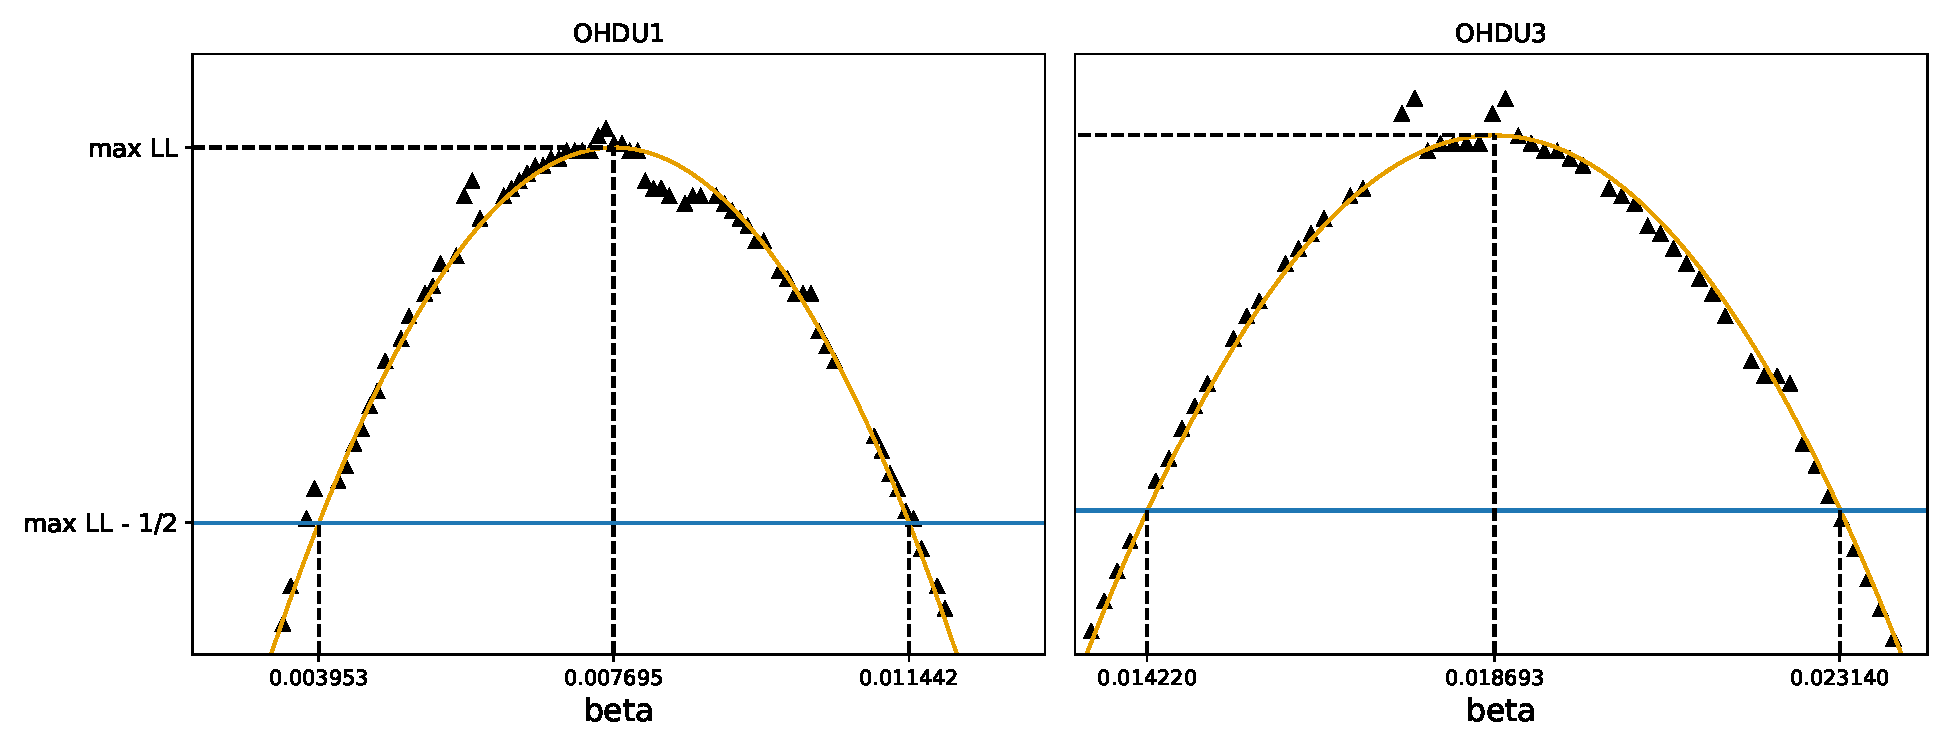
\includegraphics[scale=0.5]{Figs/Al_barridos_beta.pdf}
    \caption{Curvas del logaritmo de la verosimilitud en función de $\beta$, para los cuadrantes uno y tres con rayos $X$ del aluminio. Del ajuste cuadrático se obtiene el $\hat{\beta}$ máximo y de su intersección con la recta a altura $\ln{(\Lagr(\hat{\beta}))} - 1/2$, los extremos de los intervalos.}
    \label{fig:Al_barridos_beta}
\end{figure}

En los gráficos de la Figura \ref{fig:Al_OHDU1y3_EPIX15_Corr} se pueden ver los histogramas de carga con su ajuste, provenientes de la interacción con el detector de los rayos $X$ emitidos por el aluminio, obtenidos a partir de los datos a los que se les aplicó el umbral y las correcciones. El ajuste no bineado se calculó utilizando el valor de $\hat{\beta}$, que sale del barrido anterior, para derivar el $F$ y $\varepsilon_{\eh}$ óptimos. Además, en cada gráfico se encuentran superpuestos dos histogramas de carga: el histograma de carga con umbral \verb|EPIX=1.5| y, encima de este, el histograma de carga con el umbral \verb|EPIX=1.5| más las correcciones, con el fin de poder identificar si existiesen diferencias apreciables entre ambos, lo cual no sucede.
\begin{figure}[h]
    \centering
        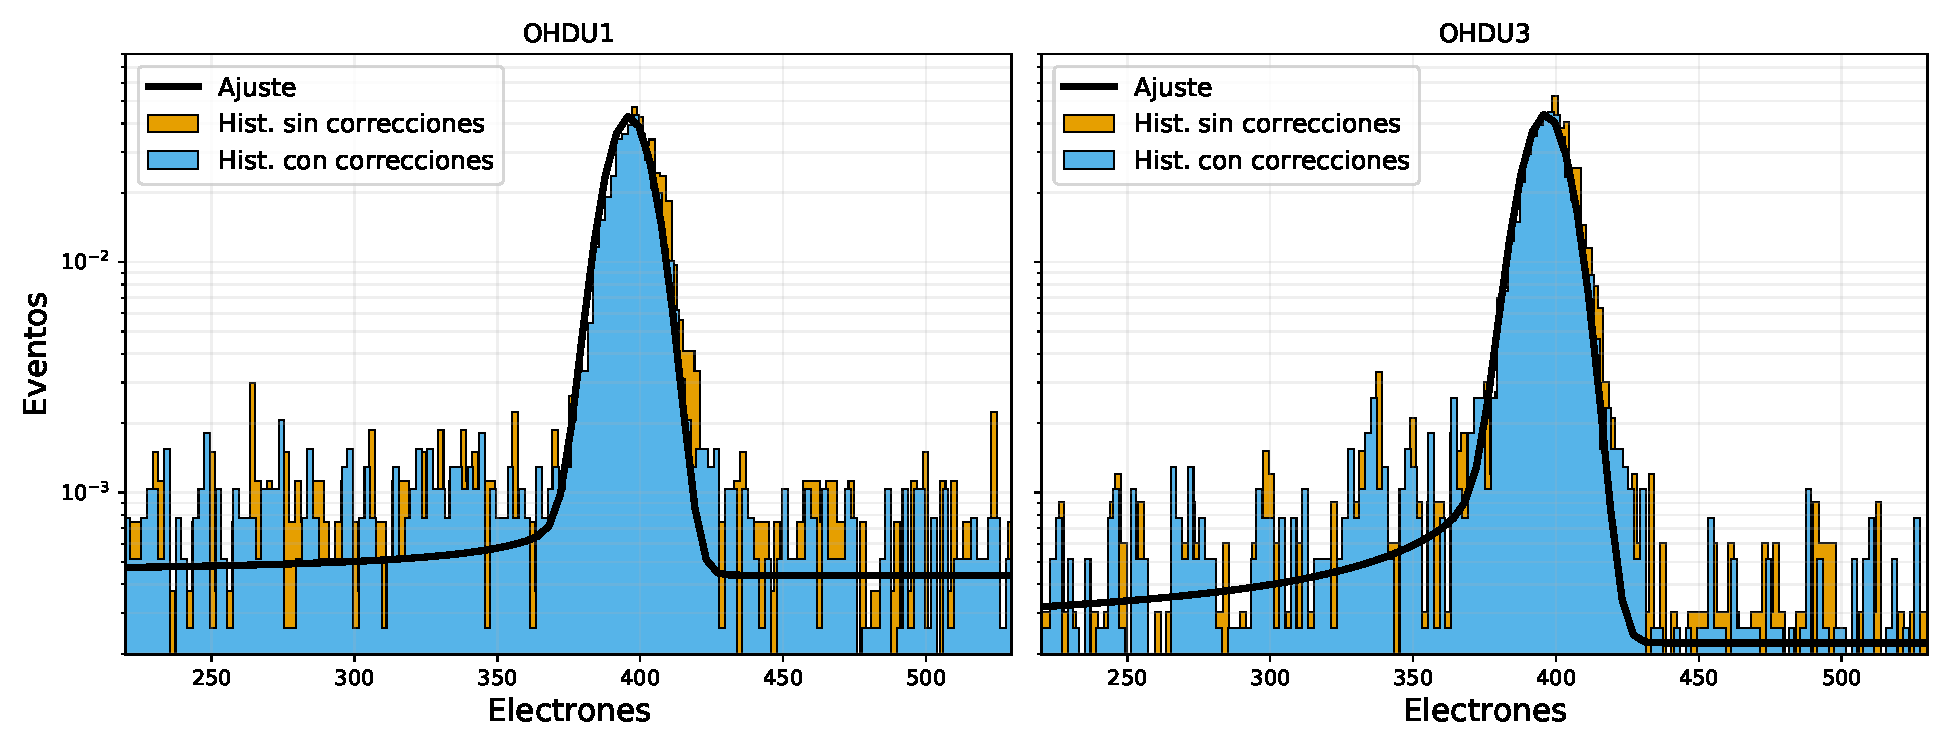
\includegraphics[scale=0.5]{Figs/Al_hists_ohdu1y3_dobles.pdf}
    \caption{Histogramas y ajustes del pico de los rayos $X$ del aluminio utilizando el modelo. El efecto de la colección parcial de carga es leve pero apreciable. Se superpusieron ambos histogramas de carga, con el nuevo umbral y con el umbral más las correcciones, en un mismo gráfico. No hay diferencias significativas en los histogramas.}
    \label{fig:Al_OHDU1y3_EPIX15_Corr}
\end{figure}

Los valores óptimos obtenidos de los ajustes se encuentran condensados en la Tabla \ref{tab:Al_FanoEehOHDU1y3}.
\begin{table}[h]
\centering
\begin{tabular*}{\textwidth}{c @{\extracolsep{\fill}} ccccc}
%\begin{tabular}{@{}ccccc@{}}
\toprule
                & \multicolumn{2}{c}{OHDU1}                 & \multicolumn{2}{c}{OHDU3}                 \\ \hline\hline
                & $F$                 & $\varepsilon_{\eh}$ & $F$                 & $\varepsilon_{\eh}$ \\
EPIX 0.5 & $0.1322 \pm 0.0022$ & $3.7141 \pm 0.0019$ & $0.1498 \pm 0.0101$ & $3.7209 \pm 0.0029$ \\ 
EPIX 1.5 & $0.1455 \pm 0.0098$ & $3.7379 \pm 0.0024$ & $0.1699 \pm 0.0150$ & $3.7419 \pm 0.0039$ \\ 
EPIX 1.5 Corr & $0.1464 \pm 0.0096$ & $3.7501 \pm 0.0006$ & $0.1504 \pm 0.0011$ & $3.7485 \pm 0.0039$ \\ \bottomrule \hline
\end{tabular*}
\caption{Magnitudes de interés obtenidas del ajuste de los histogramas de carga de los rayos $X$ del aluminio para cada uno de los pasos del análisis. El primer paso es con el umbral \texttt{EPIX=0.5}, el segundo paso es con el umbral \texttt{EPIX=1.5} y el tercer paso agrega las correcciones a la carga de los clusters.}
\label{tab:Al_FanoEehOHDU1y3}
\end{table}
%\textcolor{red}{Todos los cambios en las incertezas están dominados por la convergencia o no de la minimización, no me queda claro que respondan a la estadística. Yo no haría tanta discusión sobre este punto}
De esta se puede ver que el valor del factor de Fano aumenta $\sim 10\%$ al pasar de \verb|EPIX=0.5| a \verb|EPIX=1.5|, mientras que para el tercero el factor de Fano aumenta $\sim 13\,\%$.
%De esta se puede ver que el valor del factor de Fano aumenta al pasar de \verb|EPIX=0.5| a \verb|EPIX=1.5|, al mismo tiempo que sus incertezas, tanto para el primer cuadrante como para el tercero, lo cual no era un resultado anticipable dado el aumento de estadística. El factor de Fano aumenta $\sim 10\,\%$ y su incerteza aumenta más de $4$ veces para el primer cuadrante, mientras que para el tercero el factor de Fano aumenta $\sim 12\,\%$y su incerteza un $\sim 50\,\%$.
Al aplicar las correcciones respecto al paso anterior lo que se obtiene es una ligera disminución del valor del Fano para el primer cuadrante, alrededor del $5\,\%$, y otra no tan ligera disminución para el tercero, cerca del $\sim 12\,\%$.%, donde curiosamente las incertezas no se comportan de la misma manera para ambos casos: para el primer cuadrante la incerteza aumenta levemente, $\sim 3\,\%$, mientras que para el tercero disminuye muchísimo, mas del $\sim 95\,\%$.
En cuanto a la energía de creación electrón-hueco, pasar de \verb|EPIX=0.5| a \verb|EPIX=1.5| y luego aplicar las correcciones, corresponde a una variación total en su valor menor al $1\%$, tanto para el primer cuadrante como para el tercero. Todo esto puede verse con mayor claridad en los gráficos inferiores de la Figura \ref{fig:Al_mu_sigma_fano_eh}.
%Al aplicar las correcciones respecto al paso anterior lo que se obtiene es una ligera disminución del valor del Fano para el primer cuadrante, menor al $1\,\%$, y otra no tan ligera disminución para el tercero, cerca del $\sim 12\,\%$, donde curiosamente las incertezas no se comportan de la misma manera para ambos casos: para el primer cuadrante la incerteza aumenta levemente, $\sim 3\,\%$, mientras que para el tercero disminuye muchísimo, mas del $\sim 95\,\%$.
Cabe destacar que tanto los valores del factor de Fano como la energía de creación electrón-hueco se solapan con su error de forma que los resultados para ambos cuadrantes resultan compatibles. 

Por otro lado, de observar el gráfico del factor de Fano y la dispersión de los picos en la Figura \ref{fig:Al_mu_sigma_fano_eh}, se puede notar que el aumento en el valor de $F$ al aplicar el umbral se debe a un aumento de $\sigma$, lo que significa que la tendencia del factor de Fano es mayormente regida por esta. Por su lado, la energía de creación electrón hueco acompaña claramente la tendencia contraria que sigue el valor medio de carga y esto se debe a que la forma en la que se la calcula es a partir de esta, como el cociente entre la energía inicial y el valor medio de carga, el cual está muy bien determinado.

También se puede notar que el aumento en la estadística y las correcciones implementadas compatibilizaron los resultados entre cuadrantes dado que sus incertezas se solapan tanto para $F$ como para $\varepsilon_{\eh}$ y sus valores absolutos difieren menos del $3\,\%$ y del $0.1\,\%$ respectivamente.
\begin{figure}[h]
    \centering
        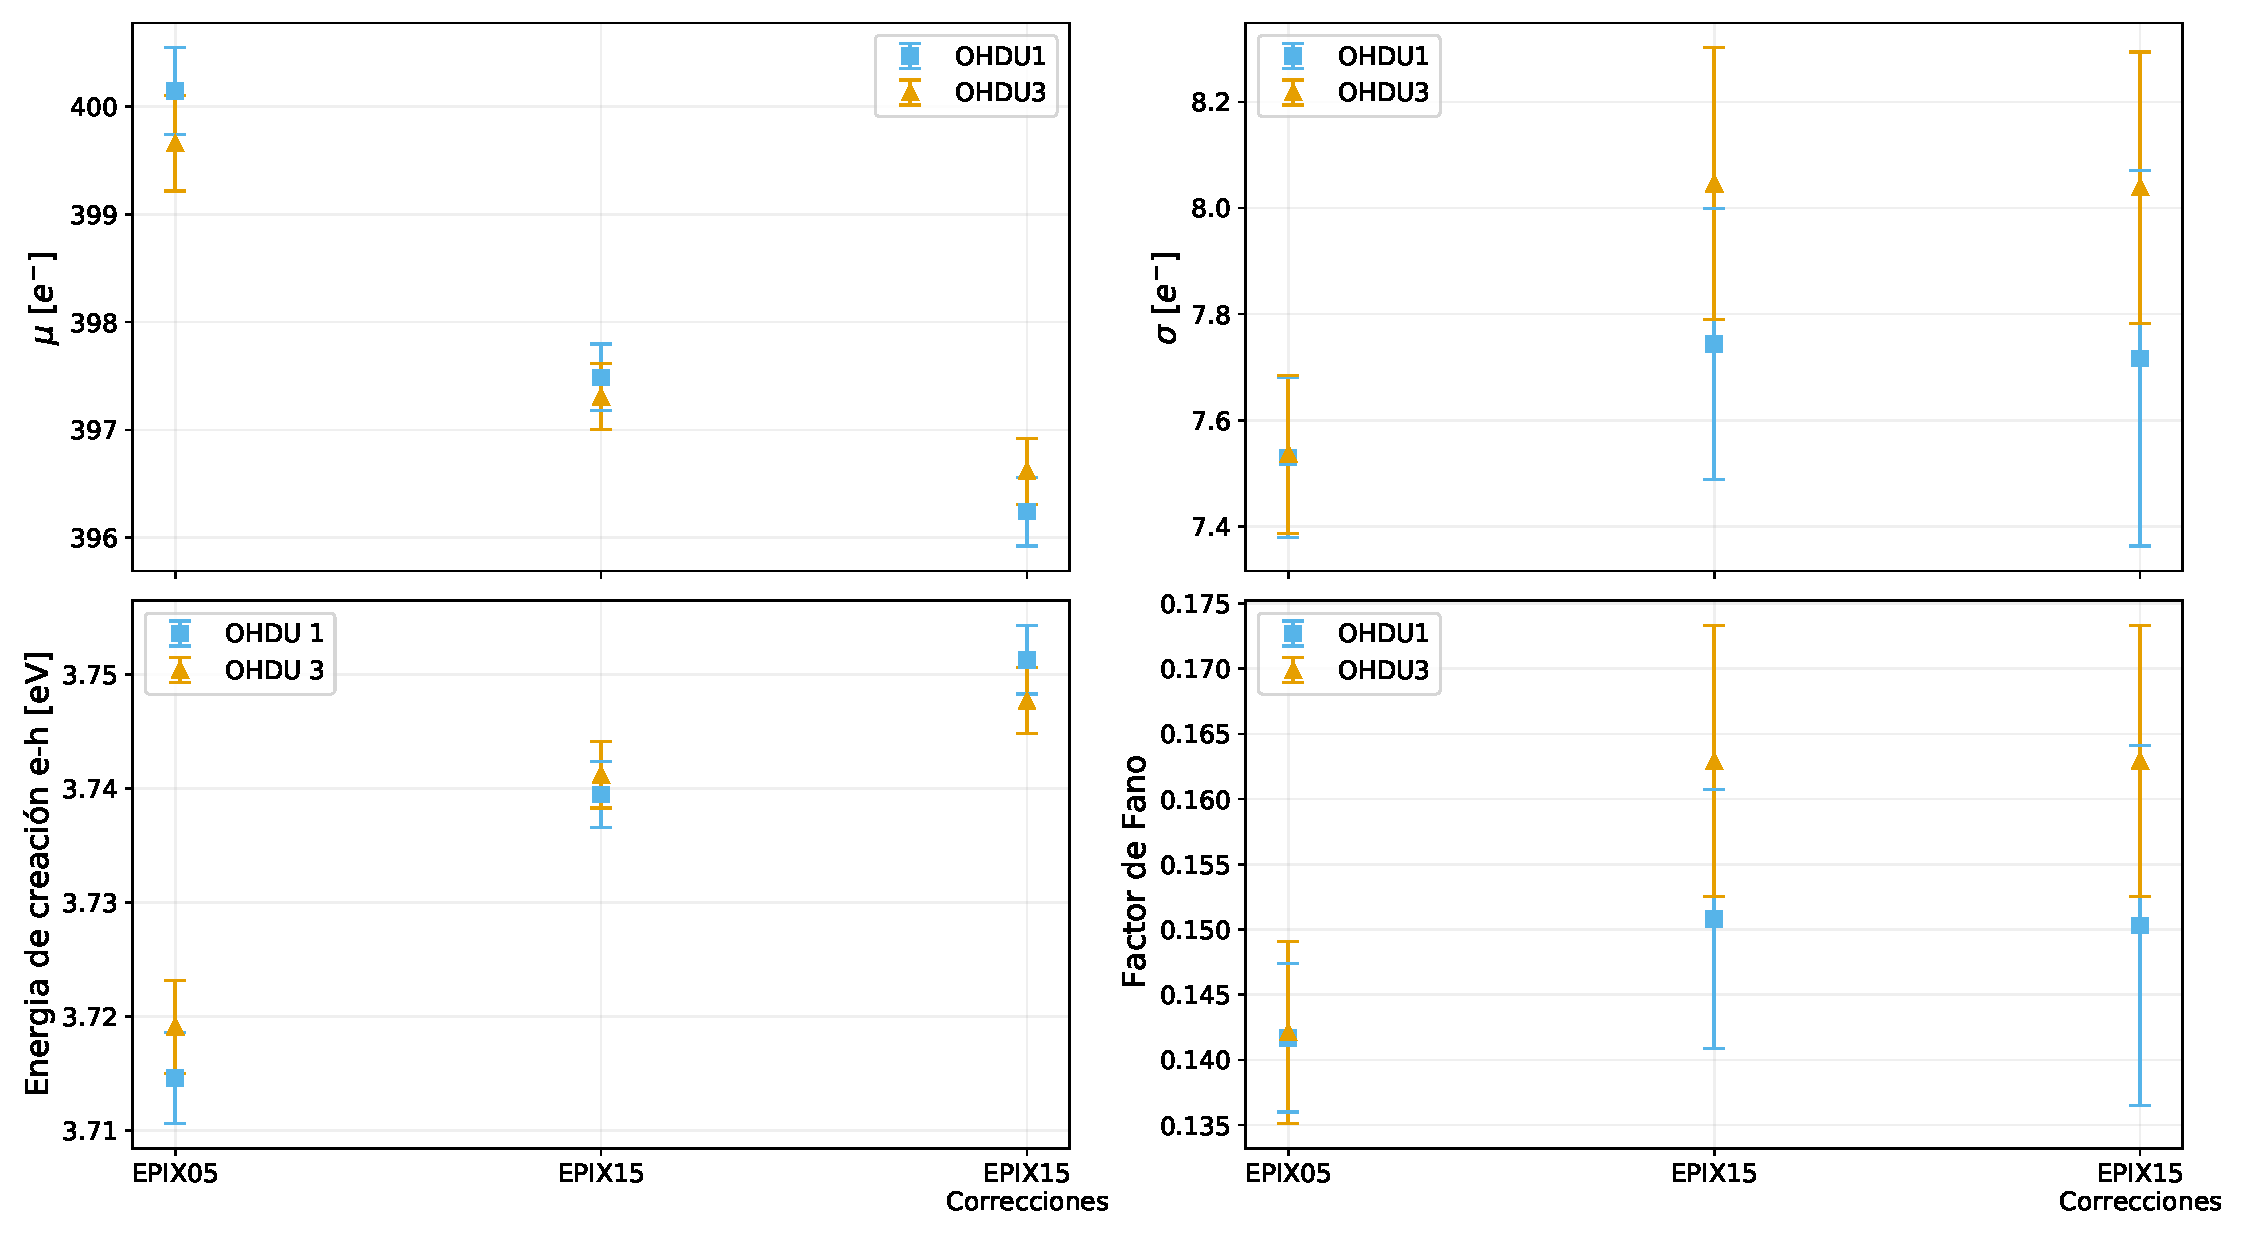
\includegraphics[scale=0.45]{Figs/Al_mu_sigma_fano_Eeh.pdf}
    \caption{Izquierda-arriba: Valor medio del pico de rayos $X$ del aluminio; izquierda-abajo: Energía de creación electrón hueco; derecha-arriba: Dispersión de los picos; derecha-abajo: factor de Fano; todas estas con sus respectivas barras de error. Se observa que la tendencia del factor de Fano es la misma que la dispersión de los picos y que la energía de creación electrón-hueco sigue la tendencia contraria al valor medio, lo cual es esperado porque se calcula a partir de esta.}
    \label{fig:Al_mu_sigma_fano_eh}
\end{figure}

Por último, los valores finales para el factor de Fano y la energía de creación electrón-hueco se obtienen de hacer el promedio pesado de los resultados de ambos cuadrantes con sus incertezas. Para el factor de Fano se obtiene $ F = 0.1503 \pm 0.0011 $, mientras que para la energía de creación electrón-hueco se obtiene $\varepsilon_{\eh} = 3.7501 \pm 0.0006 $.
%%%%%%%%%%%%%%%%%%%%%%%%%%%%%%%%%%%%%%%%%%%%%%%%%%%%%%%%%%%%%%%%%%
%%%%%%%%%%%%%%%%%%%%%%%%%%%%%%%%%%%%%%%%%%%%%%%%%%%%%%%%%%%%%%%%%%
%\pagebreak
\subsection{Resultados a 677 keV (F)}
\noindent Repitiendo el análisis llevado a cabo para el aluminio, se realizaron barridos en $\beta$ para obtener las curvas del logaritmo de la verosimilitud con su ajuste cuadrático, de las cuales se obtienen el $\hat{\beta}$ máximo y los extremos de su intervalo de confianza en cada cuadrante, como se ve en la Figura \ref{fig:F_barridos_beta}. Para el primer cuadrante, del ajuste se desprende $\hat{\beta} = 0.0927 $, con su intervalo $[0.0842;\ 0.1013]$ y para el tercer cuadrante se obtiene $\hat{\beta} = 0.1123 $ con su intervalo $[0.1048;\ 0.1194]$. Nuevamente, calculando el promedio pesado se obtiene $\hat{\beta} = 0.1041 \pm 0.0055 $. La primera diferencia que se tiene entre el flúor y el aluminio es que el valor de $\hat{\beta}$ del flúor resulta un orden de magnitud mayor que el del aluminio.

En este caso, sabiendo que la longitud de atenuación en el silicio para los rayos $X$ del flúor de $677\,\si{eV}$ es de $\tau_{\scaleto{X}{4pt}} = 0.941\,\si{\mu m}$\cite{AttenuationLength}, se obtiene que el ancho de la región de PCC del detector es de $\tau_{\scaleto{CCE}{4pt}} = (0.0979 \pm 0.0052)\,\si{\mu m}$, resultado muy compatible con el obtenido para el aluminio.
\begin{figure}[h]
    \centering
    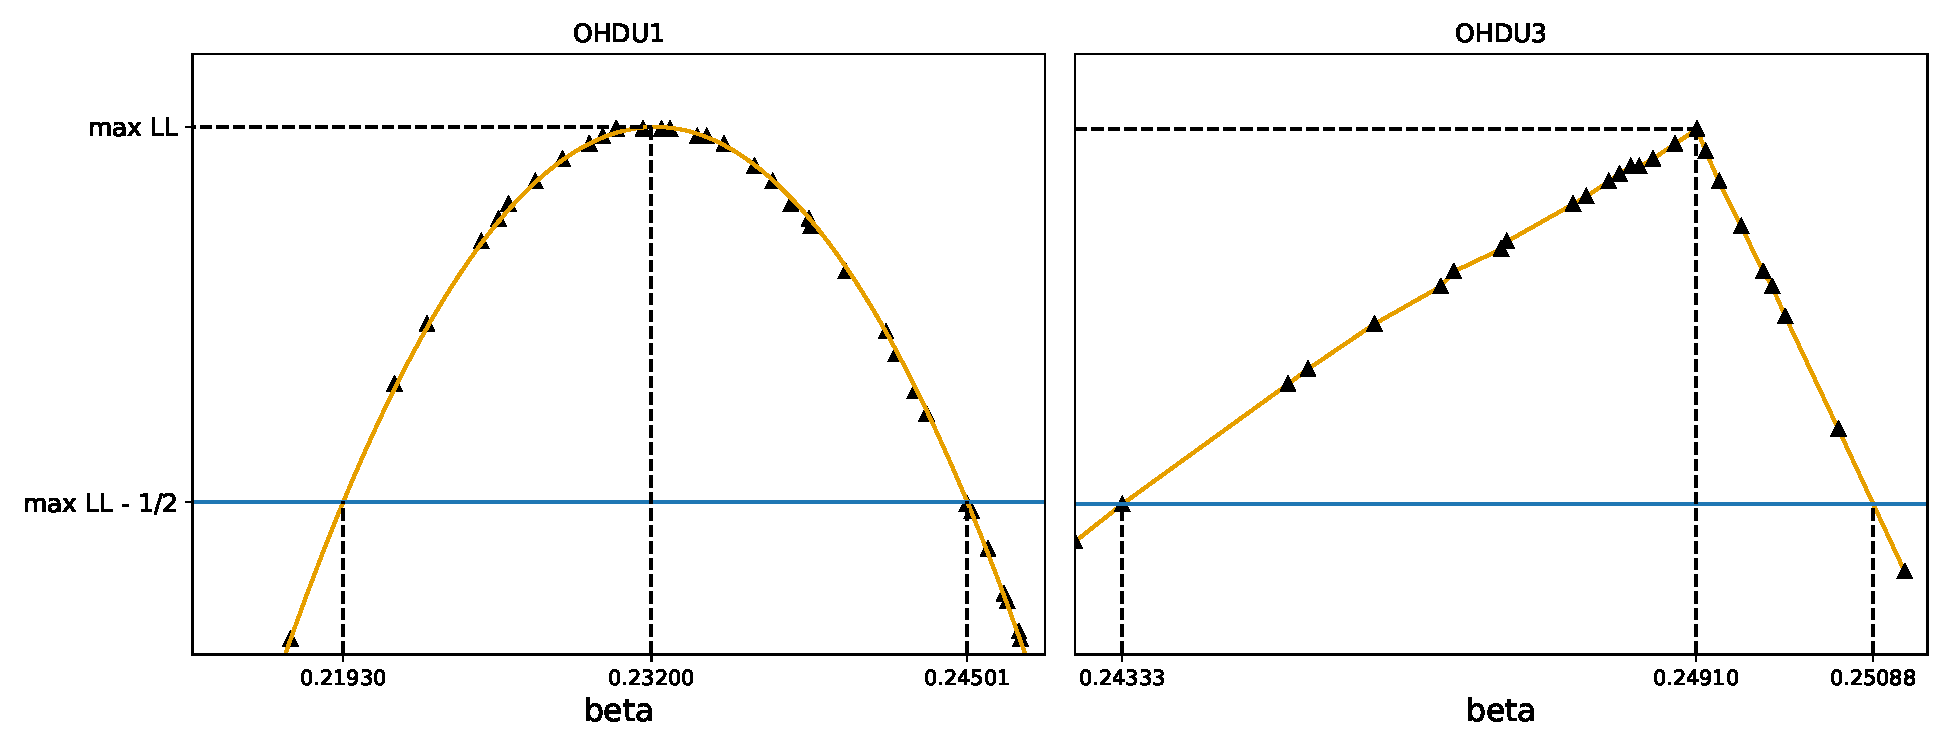
\includegraphics[scale=0.5]{Figs/F_barridos_beta.pdf}
    \caption{Curvas del logaritmo de la verosimilitud en función de $\beta$, para los cuadrantes uno y tres con rayos $X$ del flúor. Del ajuste cuadrático del primer cuadrante se obtiene el $\hat{\beta}$ máximo y de su intersección con la recta a a altura $\ln{(\Lagr(\hat{\beta}))} - 1/2$, los extremos de los intervalos. La curva para el tercer cuadrante no resultó ser cuadrática por lo cual no se realizó su ajuste, sin embargo se determina el intervalo dado por la intersección entre la recta a distancia $1/2$ de su máximo y la recta que une a los puntos que se encuentran de un lado y del otro de esta.}
    \label{fig:F_barridos_beta}
\end{figure}

Por otro lado, con el valor $\hat{\beta}$ hallado a partir de los barridos anteriores, se realizaron los ajustes no bineados a los histogramas de carga de ambos cuadrantes y se obtuvieron los valores para el factor de Fano y energía de creación electrón-hueco óptimos. De la misma forma que para el aluminio, en la Figura \ref{fig:F_OHDU1y3_EPIX15conCorr} se tienen los histogramas de carga para el primer y el tercer cuadrante, con y sin corrección, y con su respectivo ajuste. Se observa como la colección parcial de carga afecta a estos picos de forma mucho más importante que para el aluminio, formando colas muy pronunciadas a la izquierda de estos. Esto es un resultado que se anticipaba en el Capítulo \ref{chap:ModeloPCC} y se debe al aumento del valor del parámetro $\beta$: como la longitud de atenuación para los rayos $X$ del flúor es mucho menor que la del aluminio, hay muchísimos más eventos que sufren recombinación en la región de PCC del sensor. En cuanto al ajuste, para este valor de $\beta$ se ve como la curva sigue muy bien las colas de los histogramas, tanto del lado izquierdo donde hay muchos eventos, como del lado derecho donde hay muchos menos. 
\begin{figure}[h]
    \centering
    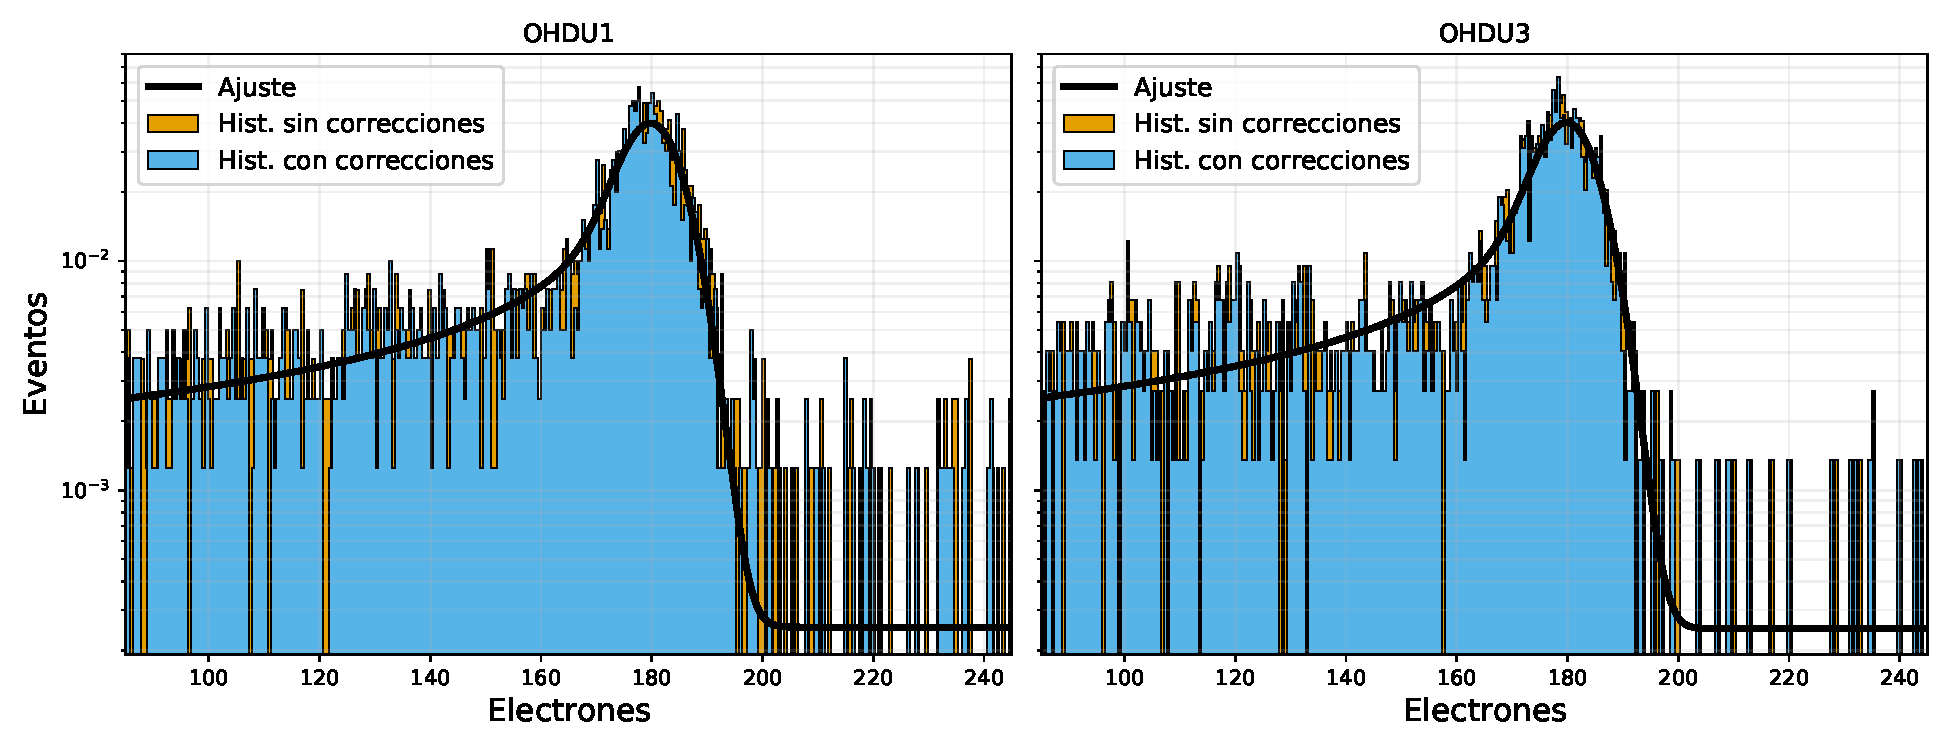
\includegraphics[scale=0.5]{Figs/F_hists_ohdu1y3_dobles.pdf}
    \caption{Histogramas y ajustes del pico de los rayos $X$ del flúor utilizando el modelo. El efecto de la colección parcial de carga es mucho más relevante en este caso, con gran cantidad de eventos a la izquierda del máximo del pico. Nuevamente se superponen ambos histogramas: con el umbral \texttt{EPIX=1.5} con y sin correcciones en un mismo gráfico. No hay se observan diferencias significativas ambos.}
    \label{fig:F_OHDU1y3_EPIX15conCorr}
\end{figure}

En la Tabla \ref{tab:F_FanoEehOHDU1y3} se presentan los resultados óptimos obtenidos de los ajustes, para los tres pasos del análisis para los cuadrantes uno y tres.
\begin{table}[h]
\centering
\begin{tabular*}{\textwidth}{c @{\extracolsep{\fill}} ccccc}
%\begin{tabular}{@{}ccccc@{}}
\toprule
                & \multicolumn{2}{c}{OHDU1}                 & \multicolumn{2}{c}{OHDU3}                 \\ \hline\hline
                & $F$                 & $\varepsilon_{\eh}$ & $F$                 & $\varepsilon_{\eh}$ \\
EPIX 0.5 & $0.1938 \pm 0.0175 $ & $3.7152 \pm 0.0060 $ & $0.1763 \pm 0.0137 $ & $3.7587 \pm 0.0051 $ \\ 
EPIX 1.5 & $0.1742 \pm 0.0183 $ & $3.7922 \pm 0.0068 $ & $0.1690 \pm 0.0163 $ & $3.8154 \pm 0.0067 $ \\ 
EPIX 1.5 Corr & $0.1711 \pm 0.0180 $ & $3.8160 \pm 0.0068 $ & $0.1676 \pm 0.0162 $ & $3.8285 \pm 0.0066 $ \\ \bottomrule \hline
\end{tabular*}
\caption{Magnitudes obtenidas del ajuste de los histogramas de carga de los rayos $X$ del aluminio para cada uno de los pasos del análisis. El primer paso es con \texttt{EPIX=0.5}, el segundo paso es con \texttt{EPIX=1.5} y el tercer paso introduce las correcciones a la carga de los clusters.}
\label{tab:F_FanoEehOHDU1y3}
\end{table}
En ambos cuadrantes se tiene que el factor de Fano disminuye al pasar de \verb|EPIX=0.5| a \verb|EPIX=1.5|, un $\sim 10\,\%$ para el primero y menos del $4\,\% $ para el tercero. Al aplicar las correcciones, el valor disminuye levemente, menos del $2\,\%$ para el primer cuadrante y menos del $1\,\%$ para el tercero. Además los valores entre el cuadrante uno y tres se solapan con su error, compatibilizándose luego de aplicar umbral y las correcciones. Para la energía de creación electrón-hueco sucede lo mismo en ambos cuadrantes, pasar de \verb|EPIX=0.5| a \verb|EPIX=1.5| aumenta el valor de la magnitud alrededor del $2\,\%$ y luego aplicar las correcciones nuevamente hay un aumento los valores para ambos cuadrantes, en este caso menor al $1\,\%$.

En los gráficos de la Figura \ref{fig:F_mu_sigma_fano_eh} se presentan los resultados anteriormente descriptos y se ven las tendencias de los valores con sus respectivos errores para cada uno de los análisis realizados. Para el caso del factor de Fano, se puede ver que sigue la misma tendencia que la dispersión, como sucedía para el aluminio y que los errores de ambos se solapan para todos los pasos. Sin embargo, al aumentar el umbral y aplicar las correcciones los valores absolutos se acercan mucho, compatibilizándose aún más. La energía de creación electrón-hueco también se compatibiliza al aplicar el umbral y las correcciones.
\begin{figure}[h]
    \centering
        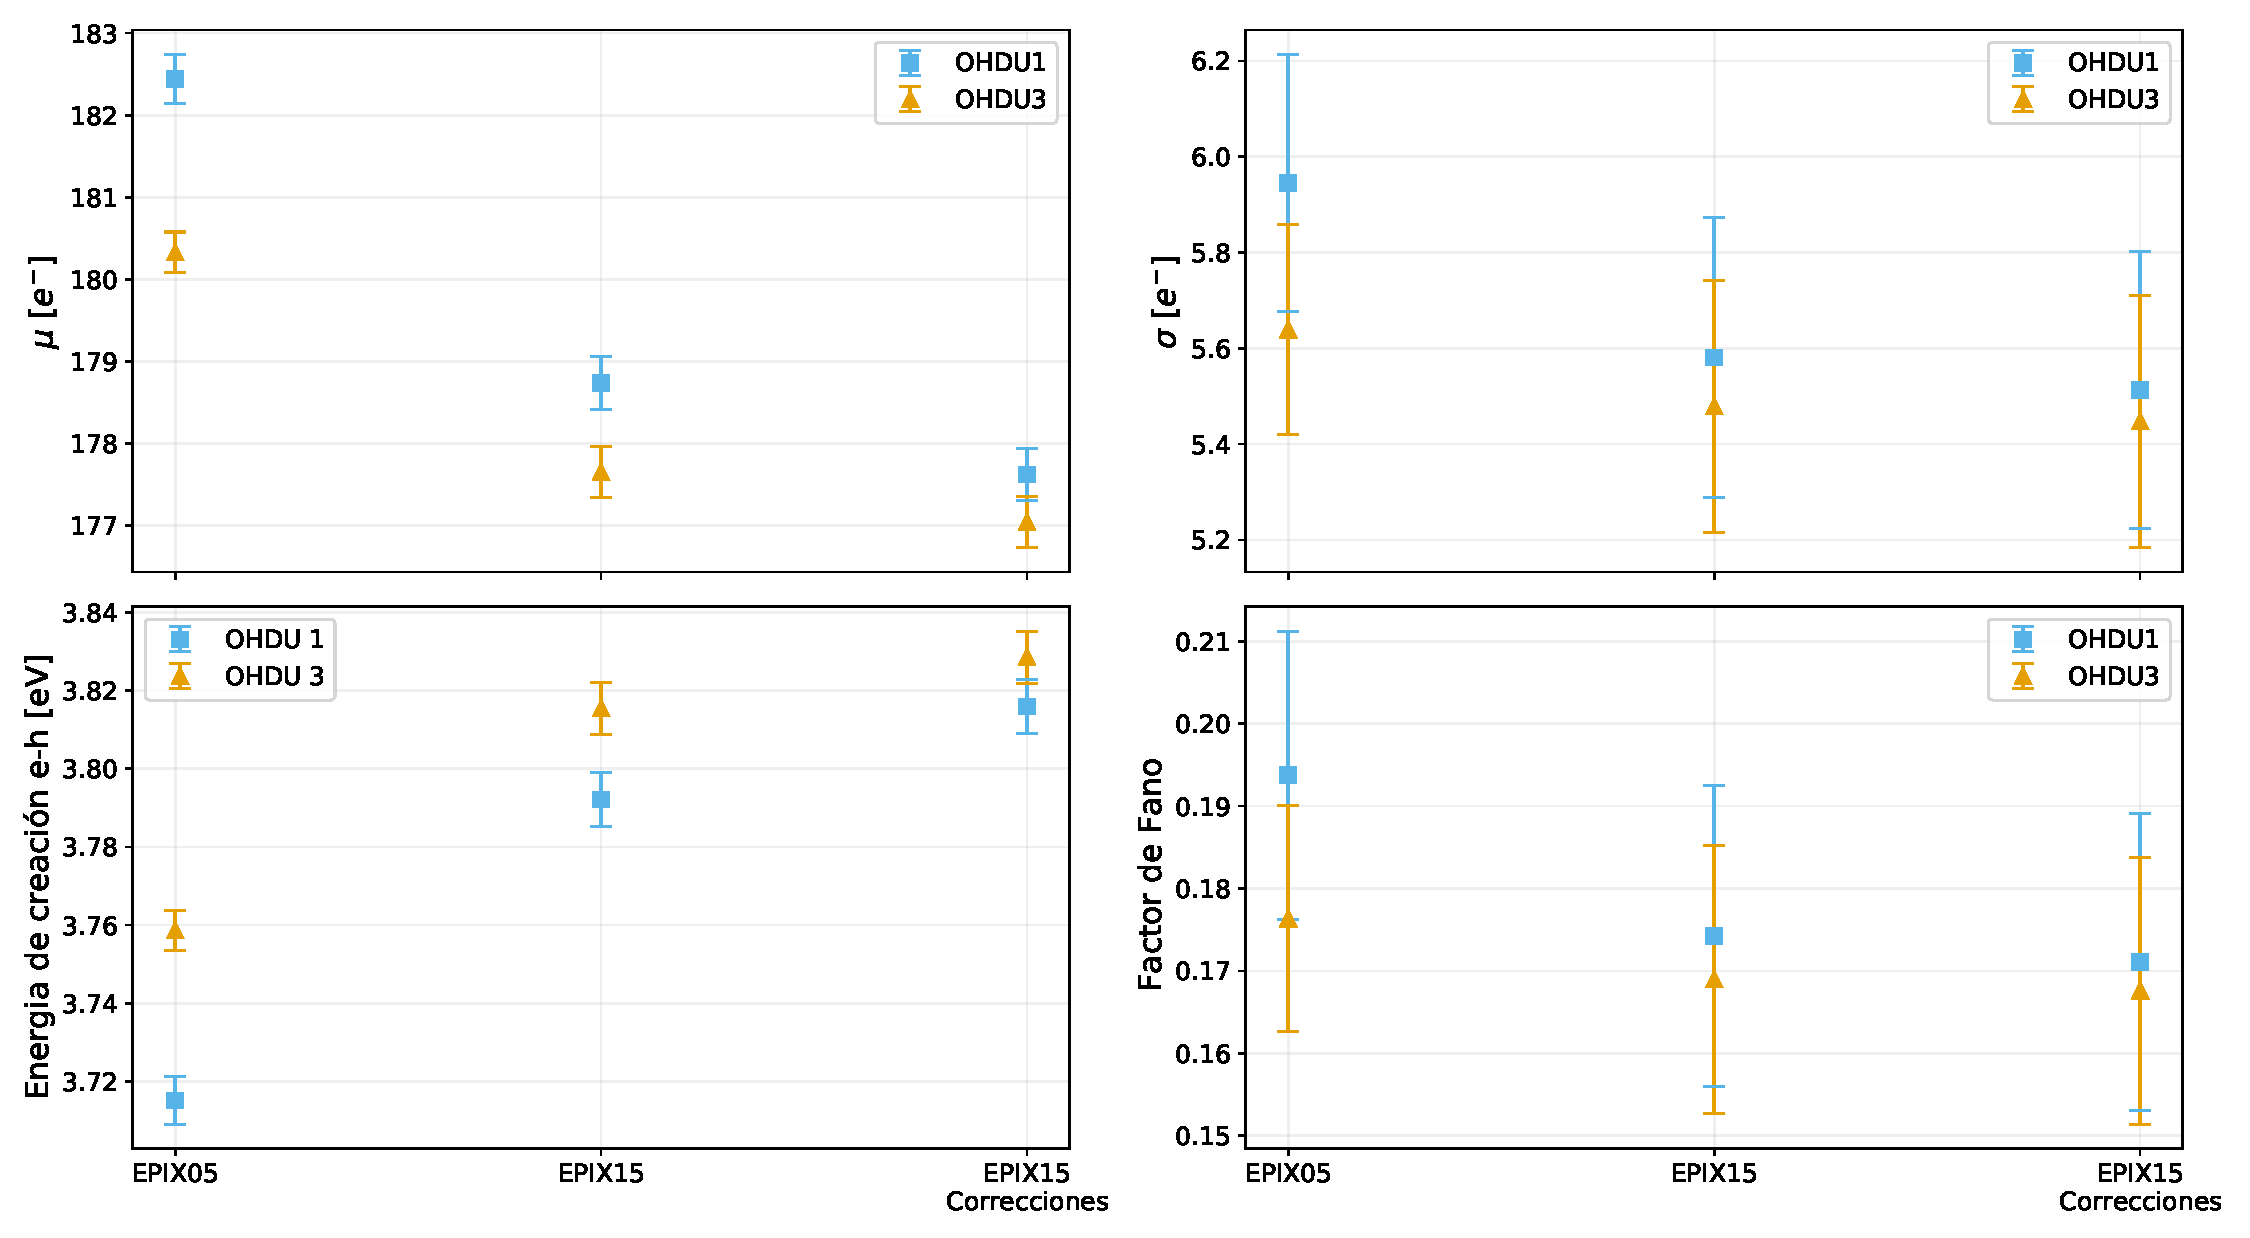
\includegraphics[scale=0.45]{Figs/F_mu_sigma_fano_Eeh.pdf}
    \caption{Izquierda-arriba: Valor medio del pico de rayos $X$ del flúor; izquierda-abajo: Energía de creación electrón hueco; derecha-arriba: Dispersión de los picos; derecha-abajo: factor de Fano; todos con sus respectivas barras de error obtenidas de los ajustes. Se observa que el factor de Fano sigue la misma tendencia que la dispersión de los picos y que la energía de creación electrón-hueco la tendencia contraria al valor medio, de la misma manera que ocurría con estas magnitudes en el caso del aluminio.}
    \label{fig:F_mu_sigma_fano_eh}
\end{figure}

Por último, los resultados finales para los rayos $X$ del flúor se obtienen de la misma manera que para el aluminio:  se realiza el promedio pesado de las magnitudes con sus incertezas. De este cálculo se obtienen $F = 0.1694 \pm 0.0120 $ y $\varepsilon_{\eh} = 3.8222 \pm 0.0048$.

Finalmente, no se obtuvieron mejoras apreciables en las incertezas de las magnitudes a pesar del aumento de la estadística como consecuencia del nuevo umbral. Sin embargo, el procedimiento utilizado para la corrección de los sesgos logra compatibilizar los cuadrantes entre sí, tanto para el factor de Fano como para el energía de creación electrón-hueco. Por otro lado, estos resultados también ponen de manifiesto la ventaja de la utilización de este nuevo modelo de ajuste, debido a que a partir de este tipo de mediciones se puede obtener el ancho efectivo de la región de colección parcial de carga del detector.

Con estos resultados se puede actualizar el gráfico de la Figura \ref{fig:Fano_y_ruido} resultando en la nueva Figura \ref{fig:Fano_y_ruido_final}, donde se ven los nuevos valores para el factor de Fano obtenidos de este trabajo, que no se posicionan sobre la recta de valor constante $F = 0.119$, correspondiente al valor reportado para los rayos $X$ del $\Fe{55}$ en trabajos anteriores\cite{Rodrigues}.
\begin{figure}[H]
    \centering
        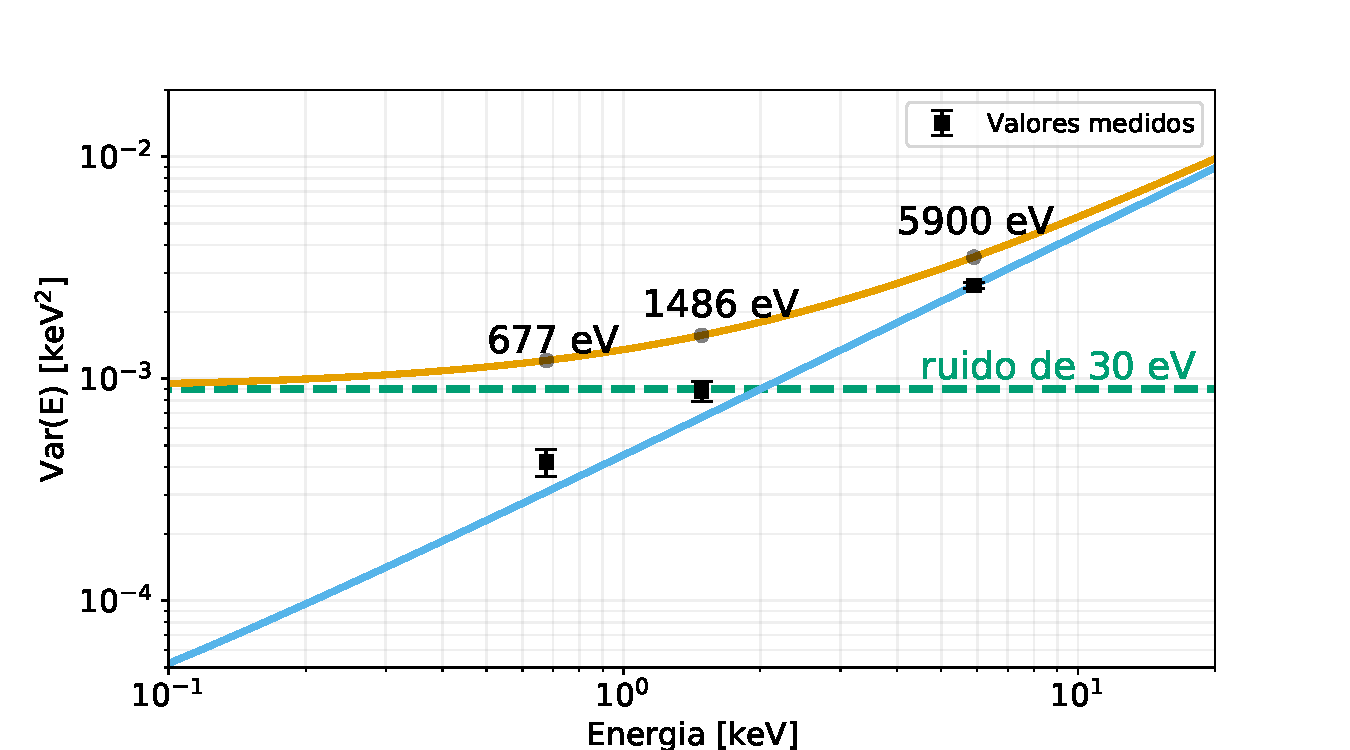
\includegraphics[scale=0.5]{Figs/FanoyRuidoFinal.pdf}
    \caption{Gráfico del factor de Fano obtenido de las mediciones y análisis realizados en este trabajo (cuadrados negros) comparado con la recta esperada si el factor de Fano fuera constante. Se observa que los valores medidos se acercan a la recta del factor de Fano constante. También se grafica la curva y los valores con lo que mediría un CCD convencional para estas energías (puntos negros).}
    \label{fig:Fano_y_ruido_final}
\end{figure}